\section{Register description}
\regover{
{\hyperref[pwm-pwm-int-config]{pwm\_int\_config}}&PWM interrupt configuration register
\\
\hline
{\hyperref[pwm-pwm0-clkdiv]{pwm0\_clkdiv}}&PWM0 clock division configuration register
\\
\hline
{\hyperref[pwm-pwm0-thre1]{pwm0\_thre1}}&PWM0 first counter threshold configuration register
\\
\hline
{\hyperref[pwm-pwm0-thre2]{pwm0\_thre2}}&PWM0 sencond counter threshold configuration register
\\
\hline
{\hyperref[pwm-pwm0-period]{pwm0\_period}}&PWM0 period setting register
\\
\hline
{\hyperref[pwm-pwm0-config]{pwm0\_config}}&PWM0 configuration register
\\
\hline
{\hyperref[pwm-pwm0-interrupt]{pwm0\_interrupt}}&PWM0 interrupt register
\\
\hline
{\hyperref[pwm-pwm1-clkdiv]{pwm1\_clkdiv}}&PWM1 clock division configuration register
\\
\hline
{\hyperref[pwm-pwm1-thre1]{pwm1\_thre1}}&PWM1 first counter threshold configuration register
\\
\hline
{\hyperref[pwm-pwm1-thre2]{pwm1\_thre2}}&PWM1 sencond counter threshold configuration register
\\
\hline
{\hyperref[pwm-pwm1-period]{pwm1\_period}}&PWM1 period setting register
\\
\hline
{\hyperref[pwm-pwm1-config]{pwm1\_config}}&PWM1 configuration register
\\
\hline
{\hyperref[pwm-pwm1-interrupt]{pwm1\_interrupt}}&PWM1 interrupt register
\\
\hline
{\hyperref[pwm-pwm2-clkdiv]{pwm2\_clkdiv}}&PWM2 clock division configuration register
\\
\hline
{\hyperref[pwm-pwm2-thre1]{pwm2\_thre1}}&PWM2 first counter threshold configuration register
\\
\hline
{\hyperref[pwm-pwm2-thre2]{pwm2\_thre2}}&PWM2 sencond counter threshold configuration register
\\
\hline
{\hyperref[pwm-pwm2-period]{pwm2\_period}}&PWM2 period setting register
\\
\hline
{\hyperref[pwm-pwm2-config]{pwm2\_config}}&PWM2 configuration register
\\
\hline
{\hyperref[pwm-pwm2-interrupt]{pwm2\_interrupt}}&PWM2 interrupt register
\\
\hline
{\hyperref[pwm-pwm3-clkdiv]{pwm3\_clkdiv}}&PWM3 clock division configuration register
\\
\hline
{\hyperref[pwm-pwm3-thre1]{pwm3\_thre1}}&PWM3 first counter threshold configuration register
\\
\hline
{\hyperref[pwm-pwm3-thre2]{pwm3\_thre2}}&PWM3 sencond counter threshold configuration register
\\
\hline
{\hyperref[pwm-pwm3-period]{pwm3\_period}}&PWM3 period setting register
\\
\hline
{\hyperref[pwm-pwm3-config]{pwm3\_config}}&PWM3 configuration register
\\
\hline
{\hyperref[pwm-pwm3-interrupt]{pwm3\_interrupt}}&PWM3 interrupt register
\\
\hline
{\hyperref[pwm-pwm4-clkdiv]{pwm4\_clkdiv}}&PWM4 clock division configuration register
\\
\hline
{\hyperref[pwm-pwm4-thre1]{pwm4\_thre1}}&PWM4 first counter threshold configuration register
\\
\hline
{\hyperref[pwm-pwm4-thre2]{pwm4\_thre2}}&PWM4 sencond counter threshold configuration register
\\
\hline
{\hyperref[pwm-pwm4-period]{pwm4\_period}}&PWM4 period setting register
\\
\hline
{\hyperref[pwm-pwm4-config]{pwm4\_config}}&PWM4 configuration register
\\
\hline
{\hyperref[pwm-pwm4-interrupt]{pwm4\_interrupt}}&PWM4 interrupt register
\\
\hline
}

\subsection{pwm\_int\_config}
\label{pwm-pwm-int-config}
Address:0x4000a400
 \begin{figure}[H]
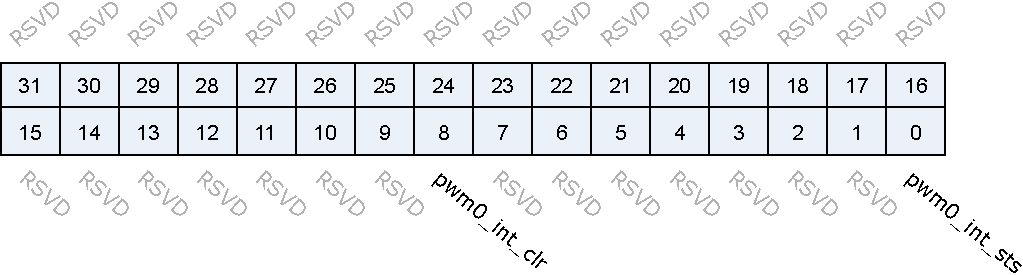
\includegraphics{pwm_pwm_int_config.pdf}
\end{figure}

\regdes{31:14&RSVD& & & \\\hline
13:8&pwm\_int\_clear&w&6'd0&PWM channel interrupt clear\\\hline
7:6&RSVD& & & \\\hline
5:0&pwm\_interrupt\_sts&r&6'd0&PWM channel interrupt status\\\hline

}
\subsection{pwm0\_clkdiv}
\label{pwm-pwm0-clkdiv}
Address:0x4000a420
 \begin{figure}[H]
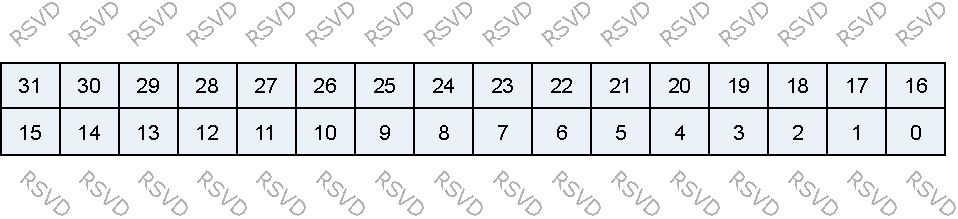
\includegraphics{pwm_pwm0_clkdiv.pdf}
\end{figure}

\regdes{31:16&RSVD& & & \\\hline
15:0&pwm\_clk\_div&r/w&16'b0&PWM clock division\\\hline

}
\subsection{pwm0\_thre1}
\label{pwm-pwm0-thre1}
Address:0x4000a424
 \begin{figure}[H]
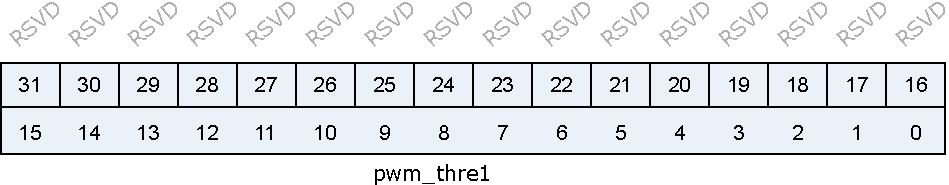
\includegraphics{pwm_pwm0_thre1.pdf}
\end{figure}

\regdes{31:16&RSVD& & & \\\hline
15:0&pwm\_thre1&r/w&16'b0&PWM first counter threshold, can't be larger that pwm\_thre2\\\hline

}
\subsection{pwm0\_thre2}
\label{pwm-pwm0-thre2}
Address:0x4000a428
 \begin{figure}[H]
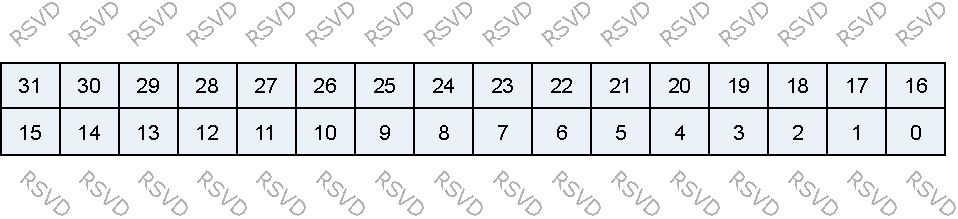
\includegraphics{pwm_pwm0_thre2.pdf}
\end{figure}

\regdes{31:16&RSVD& & & \\\hline
15:0&pwm\_thre2&r/w&16'd0&PWM sencond counter threshold, can't be smaller that pwm\_thre1\\\hline

}
\subsection{pwm0\_period}
\label{pwm-pwm0-period}
Address:0x4000a42c
 \begin{figure}[H]
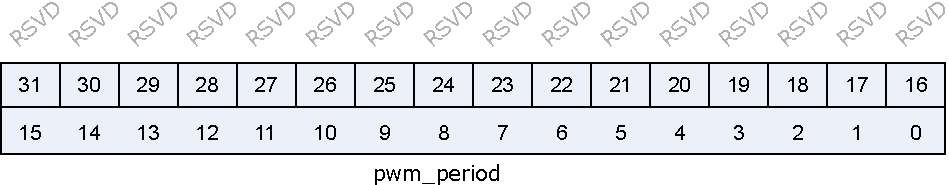
\includegraphics{pwm_pwm0_period.pdf}
\end{figure}

\regdes{31:16&RSVD& & & \\\hline
15:0&pwm\_period&r/w&16'd0&PWM period setting\\\hline

}
\subsection{pwm0\_config}
\label{pwm-pwm0-config}
Address:0x4000a430
 \begin{figure}[H]
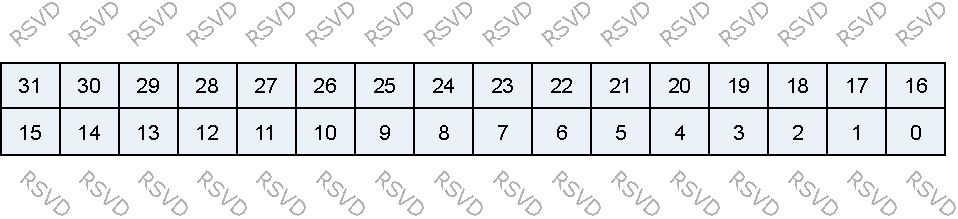
\includegraphics{pwm_pwm0_config.pdf}
\end{figure}

\regdes{31:8&RSVD& & & \\\hline
7&pwm\_sts\_top&r&1'b0&PWM stop status\\\hline
6&pwm\_stop\_en&r/w&1'b0&PWM stop enable\\\hline
5&pwm\_sw\_mode&r/w&1'b0&PWM SW Mode setting\\\hline
4&pwm\_sw\_force\_val&r/w&1'b0&PWM SW Mode force value\\\hline
3&pwm\_stop\_mode&r/w&1'b1&PWM stop mode, 1'b1 - graceful ; 1'b0 - abrupt\\\hline
2&pwm\_out\_inv&r/w&1'b0&PWM invert output mode\\\hline
1:0&reg\_clk\_sel&r/w&2'd0&PWM clock source select, 2'b00-xclk ; 2'b01-bclk ; others-f32k\_clk\\\hline

}
\subsection{pwm0\_interrupt}
\label{pwm-pwm0-interrupt}
Address:0x4000a434
 \begin{figure}[H]
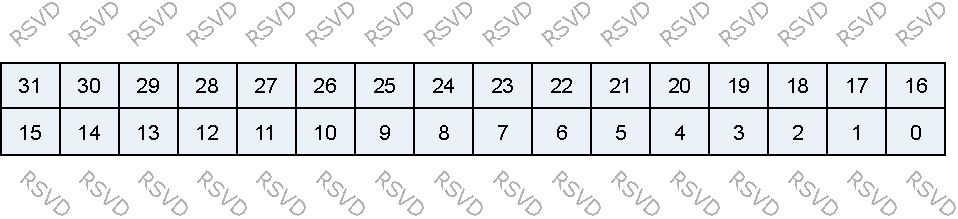
\includegraphics{pwm_pwm0_interrupt.pdf}
\end{figure}

\regdes{31:17&RSVD& & & \\\hline
16&pwm\_int\_enable&r/w&1'b0&PWM interrupt enable\\\hline
15:0&pwm\_int\_period\_cnt&r/w&16'd0&PWM interrupt period counter threshold\\\hline

}
\subsection{pwm1\_clkdiv}
\label{pwm-pwm1-clkdiv}
Address:0x4000a440
 \begin{figure}[H]
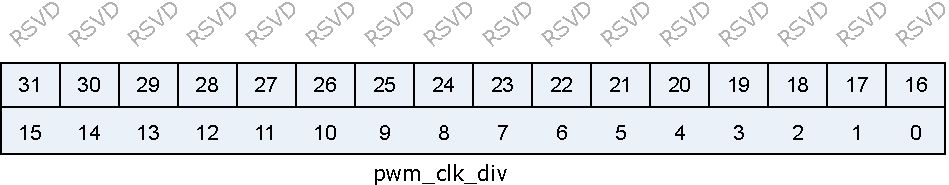
\includegraphics{pwm_pwm1_clkdiv.pdf}
\end{figure}

\regdes{31:16&RSVD& & & \\\hline
15:0&pwm\_clk\_div&r/w&16'b0&PWM clock division\\\hline

}
\subsection{pwm1\_thre1}
\label{pwm-pwm1-thre1}
Address:0x4000a444
 \begin{figure}[H]
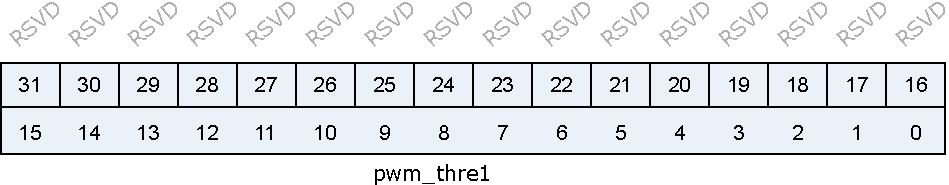
\includegraphics{pwm_pwm1_thre1.pdf}
\end{figure}

\regdes{31:16&RSVD& & & \\\hline
15:0&pwm\_thre1&r/w&16'b0&PWM first counter threshold, can't be larger that pwm\_thre2\\\hline

}
\subsection{pwm1\_thre2}
\label{pwm-pwm1-thre2}
Address:0x4000a448
 \begin{figure}[H]
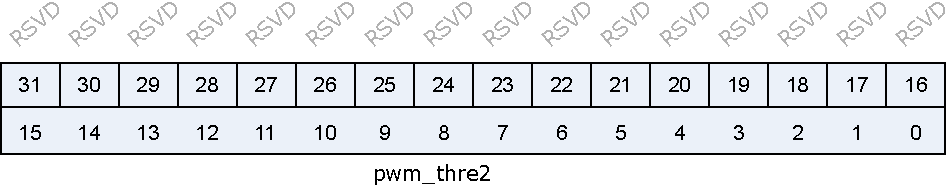
\includegraphics{pwm_pwm1_thre2.pdf}
\end{figure}

\regdes{31:16&RSVD& & & \\\hline
15:0&pwm\_thre2&r/w&16'd0&PWM sencond counter threshold, can't be smaller that pwm\_thre1\\\hline

}
\subsection{pwm1\_period}
\label{pwm-pwm1-period}
Address:0x4000a44c
 \begin{figure}[H]
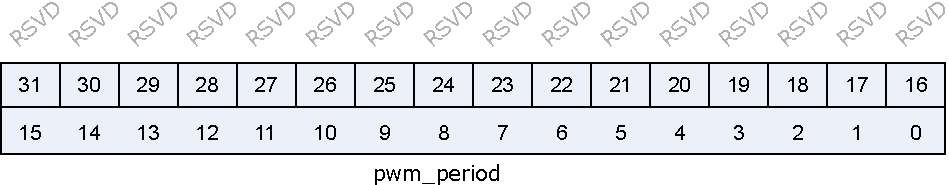
\includegraphics{pwm_pwm1_period.pdf}
\end{figure}

\regdes{31:16&RSVD& & & \\\hline
15:0&pwm\_period&r/w&16'd0&PWM period setting\\\hline

}
\subsection{pwm1\_config}
\label{pwm-pwm1-config}
Address:0x4000a450
 \begin{figure}[H]
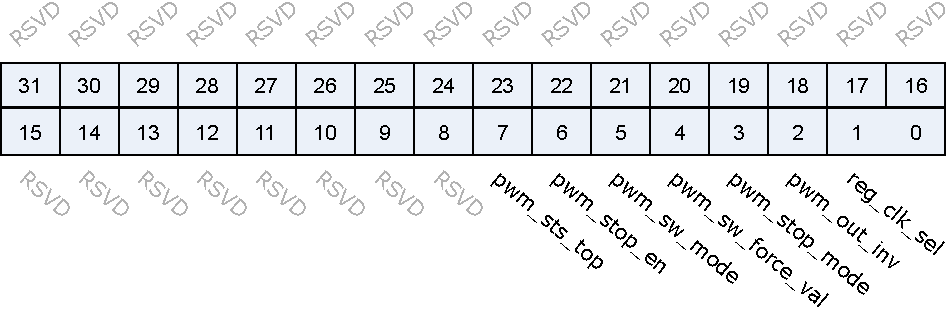
\includegraphics{pwm_pwm1_config.pdf}
\end{figure}

\regdes{31:8&RSVD& & & \\\hline
7&pwm\_sts\_top&r&1'b0&PWM stop status\\\hline
6&pwm\_stop\_en&r/w&1'b0&PWM stop enable\\\hline
5&pwm\_sw\_mode&r/w&1'b0&PWM SW Mode setting\\\hline
4&pwm\_sw\_force\_val&r/w&1'b0&PWM SW Mode force value\\\hline
3&pwm\_stop\_mode&r/w&1'b1&PWM stop mode, 1'b1 - graceful ; 1'b0 - abrupt\\\hline
2&pwm\_out\_inv&r/w&1'b0&PWM invert output mode\\\hline
1:0&reg\_clk\_sel&r/w&2'd0&PWM clock source select, 2'b00-xclk ; 2'b01-bclk ; others-f32k\_clk\\\hline

}
\subsection{pwm1\_interrupt}
\label{pwm-pwm1-interrupt}
Address:0x4000a454
 \begin{figure}[H]
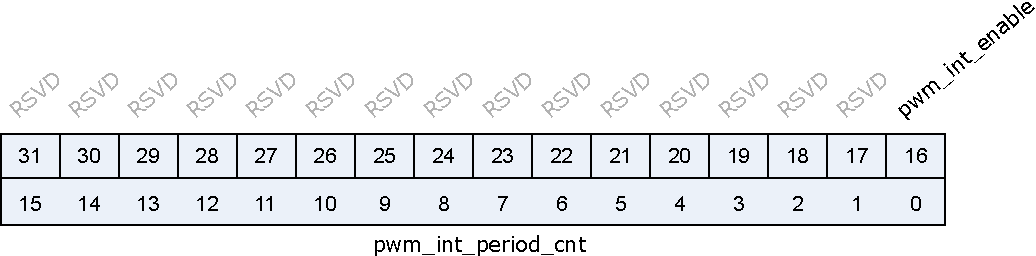
\includegraphics{pwm_pwm1_interrupt.pdf}
\end{figure}

\regdes{31:17&RSVD& & & \\\hline
16&pwm\_int\_enable&r/w&1'b0&PWM interrupt enable\\\hline
15:0&pwm\_int\_period\_cnt&r/w&16'd0&PWM interrupt period counter threshold\\\hline

}
\subsection{pwm2\_clkdiv}
\label{pwm-pwm2-clkdiv}
Address:0x4000a460
 \begin{figure}[H]
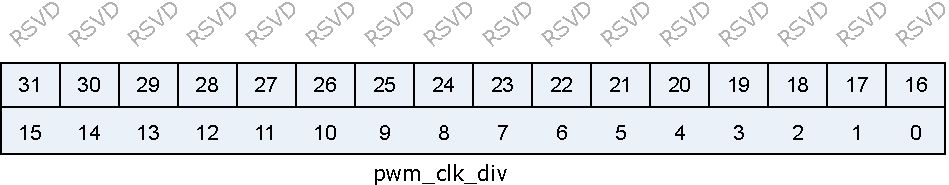
\includegraphics{pwm_pwm2_clkdiv.pdf}
\end{figure}

\regdes{31:16&RSVD& & & \\\hline
15:0&pwm\_clk\_div&r/w&16'b0&PWM clock division\\\hline

}
\subsection{pwm2\_thre1}
\label{pwm-pwm2-thre1}
Address:0x4000a464
 \begin{figure}[H]
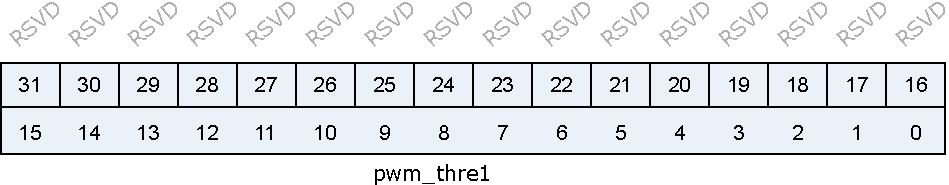
\includegraphics{pwm_pwm2_thre1.pdf}
\end{figure}

\regdes{31:16&RSVD& & & \\\hline
15:0&pwm\_thre1&r/w&16'b0&PWM first counter threshold, can't be larger that pwm\_thre2\\\hline

}
\subsection{pwm2\_thre2}
\label{pwm-pwm2-thre2}
Address:0x4000a468
 \begin{figure}[H]
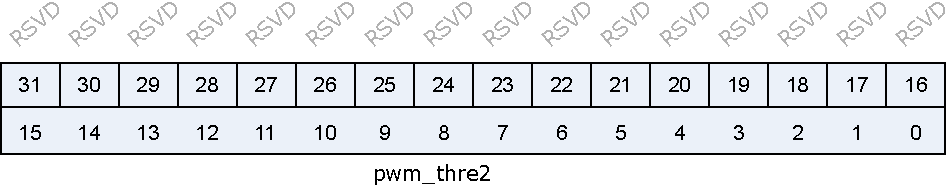
\includegraphics{pwm_pwm2_thre2.pdf}
\end{figure}

\regdes{31:16&RSVD& & & \\\hline
15:0&pwm\_thre2&r/w&16'd0&PWM sencond counter threshold, can't be smaller that pwm\_thre1\\\hline

}
\subsection{pwm2\_period}
\label{pwm-pwm2-period}
Address:0x4000a46c
 \begin{figure}[H]
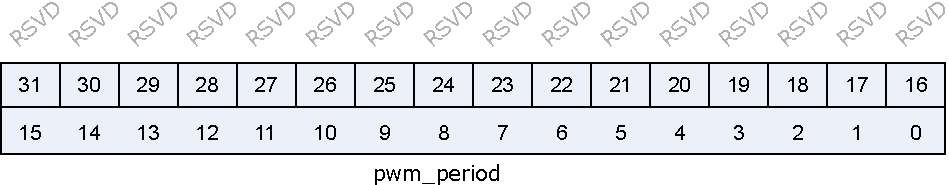
\includegraphics{pwm_pwm2_period.pdf}
\end{figure}

\regdes{31:16&RSVD& & & \\\hline
15:0&pwm\_period&r/w&16'd0&PWM period setting\\\hline

}
\subsection{pwm2\_config}
\label{pwm-pwm2-config}
Address:0x4000a470
 \begin{figure}[H]
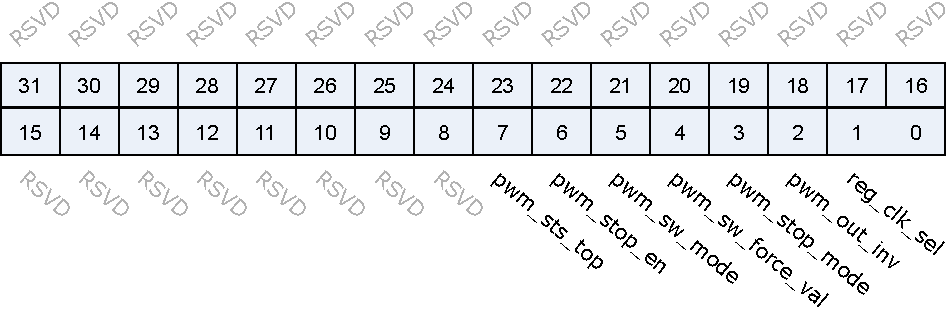
\includegraphics{pwm_pwm2_config.pdf}
\end{figure}

\regdes{31:8&RSVD& & & \\\hline
7&pwm\_sts\_top&r&1'b0&PWM stop status\\\hline
6&pwm\_stop\_en&r/w&1'b0&PWM stop enable\\\hline
5&pwm\_sw\_mode&r/w&1'b0&PWM SW Mode setting\\\hline
4&pwm\_sw\_force\_val&r/w&1'b0&PWM SW Mode force value\\\hline
3&pwm\_stop\_mode&r/w&1'b1&PWM stop mode, 1'b1 - graceful ; 1'b0 - abrupt\\\hline
2&pwm\_out\_inv&r/w&1'b0&PWM invert output mode\\\hline
1:0&reg\_clk\_sel&r/w&2'd0&PWM clock source select, 2'b00-xclk ; 2'b01-bclk ; others-f32k\_clk\\\hline

}
\subsection{pwm2\_interrupt}
\label{pwm-pwm2-interrupt}
Address:0x4000a474
 \begin{figure}[H]
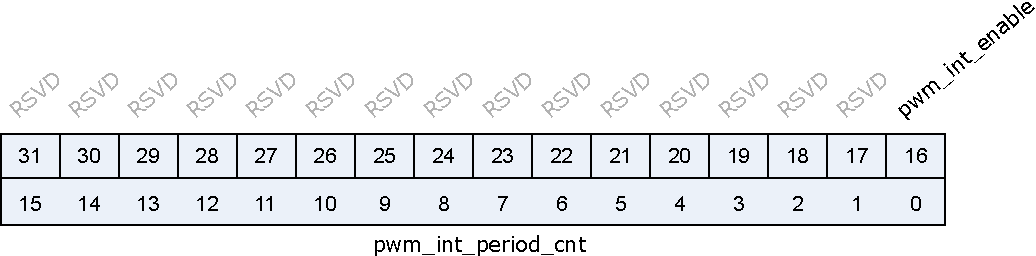
\includegraphics{pwm_pwm2_interrupt.pdf}
\end{figure}

\regdes{31:17&RSVD& & & \\\hline
16&pwm\_int\_enable&r/w&1'b0&PWM interrupt enable\\\hline
15:0&pwm\_int\_period\_cnt&r/w&16'd0&PWM interrupt period counter threshold\\\hline

}
\subsection{pwm3\_clkdiv}
\label{pwm-pwm3-clkdiv}
Address:0x4000a480
 \begin{figure}[H]
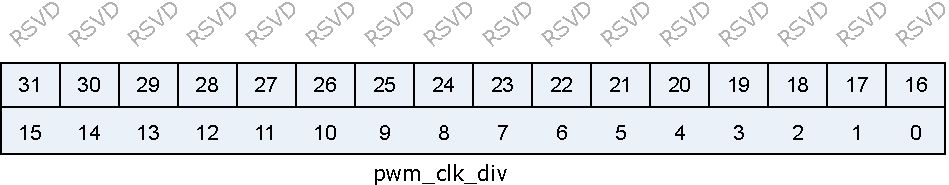
\includegraphics{pwm_pwm3_clkdiv.pdf}
\end{figure}

\regdes{31:16&RSVD& & & \\\hline
15:0&pwm\_clk\_div&r/w&16'b0&PWM clock division\\\hline

}
\subsection{pwm3\_thre1}
\label{pwm-pwm3-thre1}
Address:0x4000a484
 \begin{figure}[H]
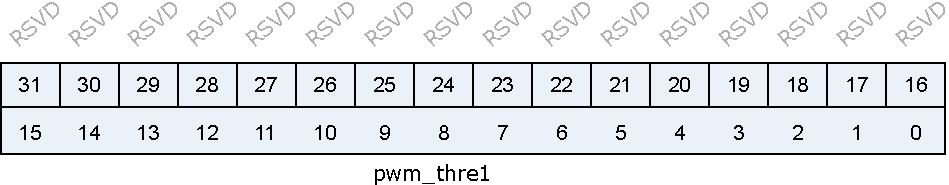
\includegraphics{pwm_pwm3_thre1.pdf}
\end{figure}

\regdes{31:16&RSVD& & & \\\hline
15:0&pwm\_thre1&r/w&16'b0&PWM first counter threshold, can't be larger that pwm\_thre2\\\hline

}
\subsection{pwm3\_thre2}
\label{pwm-pwm3-thre2}
Address:0x4000a488
 \begin{figure}[H]
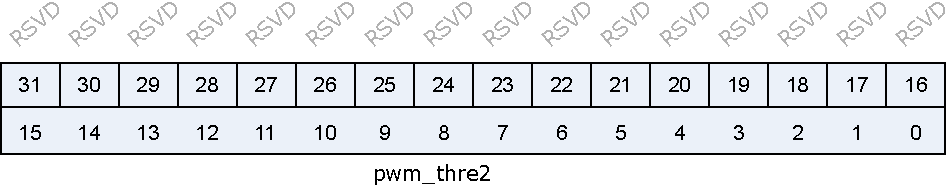
\includegraphics{pwm_pwm3_thre2.pdf}
\end{figure}

\regdes{31:16&RSVD& & & \\\hline
15:0&pwm\_thre2&r/w&16'd0&PWM sencond counter threshold, can't be smaller that pwm\_thre1\\\hline

}
\subsection{pwm3\_period}
\label{pwm-pwm3-period}
Address:0x4000a48c
 \begin{figure}[H]
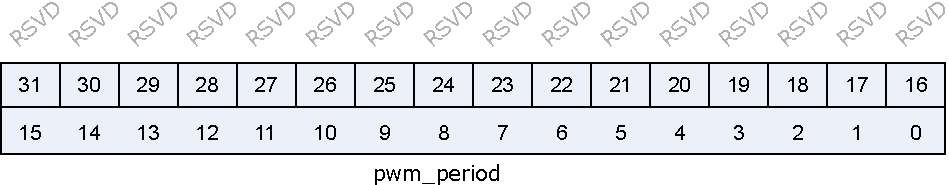
\includegraphics{pwm_pwm3_period.pdf}
\end{figure}

\regdes{31:16&RSVD& & & \\\hline
15:0&pwm\_period&r/w&16'd0&PWM period setting\\\hline

}
\subsection{pwm3\_config}
\label{pwm-pwm3-config}
Address:0x4000a490
 \begin{figure}[H]
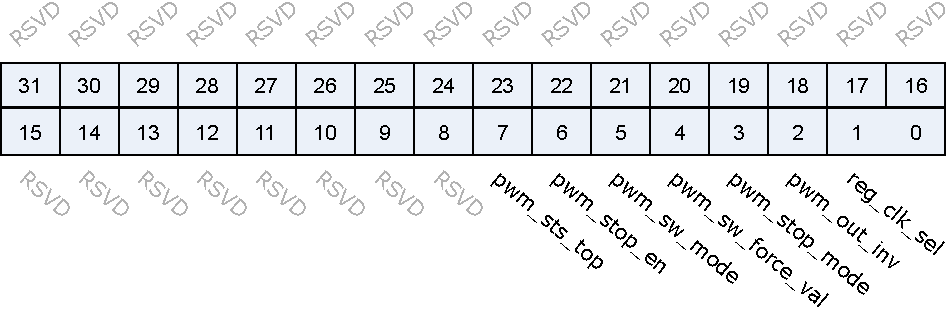
\includegraphics{pwm_pwm3_config.pdf}
\end{figure}

\regdes{31:8&RSVD& & & \\\hline
7&pwm\_sts\_top&r&1'b0&PWM stop status\\\hline
6&pwm\_stop\_en&r/w&1'b0&PWM stop enable\\\hline
5&pwm\_sw\_mode&r/w&1'b0&PWM SW Mode setting\\\hline
4&pwm\_sw\_force\_val&r/w&1'b0&PWM SW Mode force value\\\hline
3&pwm\_stop\_mode&r/w&1'b1&PWM stop mode, 1'b1 - graceful ; 1'b0 - abrupt\\\hline
2&pwm\_out\_inv&r/w&1'b0&PWM invert output mode\\\hline
1:0&reg\_clk\_sel&r/w&2'd0&PWM clock source select, 2'b00-xclk ; 2'b01-bclk ; others-f32k\_clk\\\hline

}
\subsection{pwm3\_interrupt}
\label{pwm-pwm3-interrupt}
Address:0x4000a494
 \begin{figure}[H]
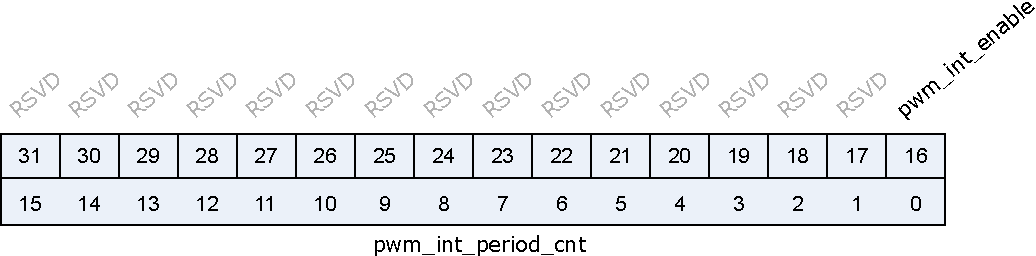
\includegraphics{pwm_pwm3_interrupt.pdf}
\end{figure}

\regdes{31:17&RSVD& & & \\\hline
16&pwm\_int\_enable&r/w&1'b0&PWM interrupt enable\\\hline
15:0&pwm\_int\_period\_cnt&r/w&16'd0&PWM interrupt period counter threshold\\\hline

}
\subsection{pwm4\_clkdiv}
\label{pwm-pwm4-clkdiv}
Address:0x4000a4a0
 \begin{figure}[H]
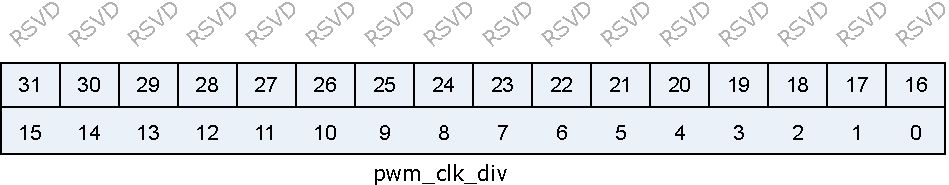
\includegraphics{pwm_pwm4_clkdiv.pdf}
\end{figure}

\regdes{31:16&RSVD& & & \\\hline
15:0&pwm\_clk\_div&r/w&16'b0&PWM clock division\\\hline

}
\subsection{pwm4\_thre1}
\label{pwm-pwm4-thre1}
Address:0x4000a4a4
 \begin{figure}[H]
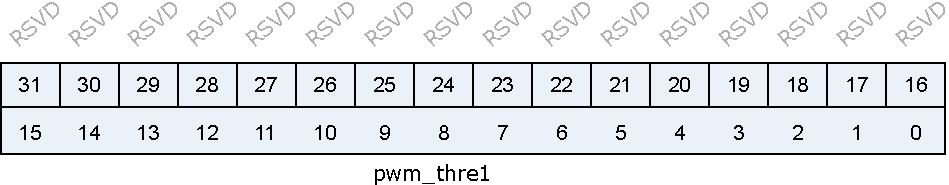
\includegraphics{pwm_pwm4_thre1.pdf}
\end{figure}

\regdes{31:16&RSVD& & & \\\hline
15:0&pwm\_thre1&r/w&16'b0&PWM first counter threshold, can't be larger that pwm\_thre2\\\hline

}
\subsection{pwm4\_thre2}
\label{pwm-pwm4-thre2}
Address:0x4000a4a8
 \begin{figure}[H]
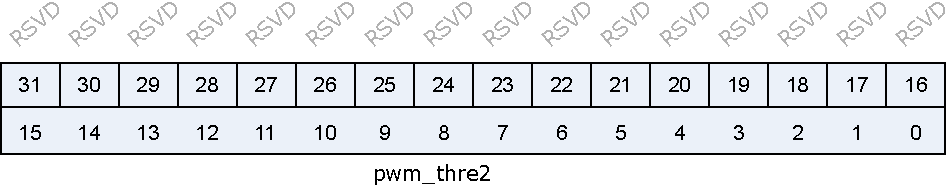
\includegraphics{pwm_pwm4_thre2.pdf}
\end{figure}

\regdes{31:16&RSVD& & & \\\hline
15:0&pwm\_thre2&r/w&16'd0&PWM sencond counter threshold, can't be smaller that pwm\_thre1\\\hline

}
\subsection{pwm4\_period}
\label{pwm-pwm4-period}
Address:0x4000a4ac
 \begin{figure}[H]
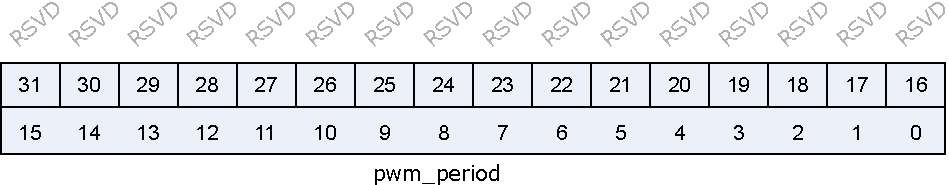
\includegraphics{pwm_pwm4_period.pdf}
\end{figure}

\regdes{31:16&RSVD& & & \\\hline
15:0&pwm\_period&r/w&16'd0&PWM period setting\\\hline

}
\subsection{pwm4\_config}
\label{pwm-pwm4-config}
Address:0x4000a4b0
 \begin{figure}[H]
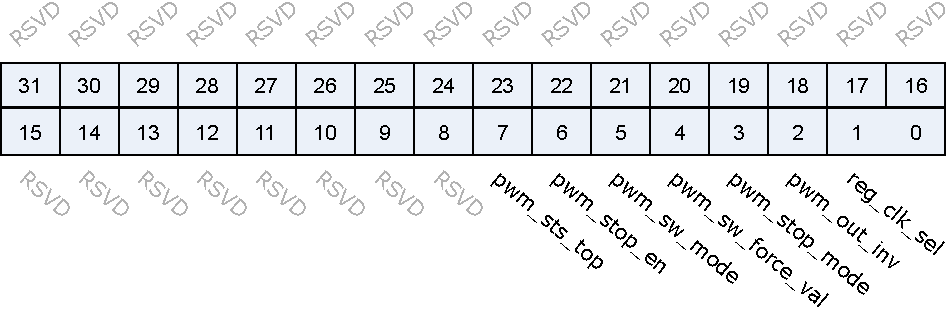
\includegraphics{pwm_pwm4_config.pdf}
\end{figure}

\regdes{31:8&RSVD& & & \\\hline
7&pwm\_sts\_top&r&1'b0&PWM stop status\\\hline
6&pwm\_stop\_en&r/w&1'b0&PWM stop enable\\\hline
5&pwm\_sw\_mode&r/w&1'b0&PWM SW Mode setting\\\hline
4&pwm\_sw\_force\_val&r/w&1'b0&PWM SW Mode force value\\\hline
3&pwm\_stop\_mode&r/w&1'b1&PWM stop mode, 1'b1 - graceful ; 1'b0 - abrupt\\\hline
2&pwm\_out\_inv&r/w&1'b0&PWM invert output mode\\\hline
1:0&reg\_clk\_sel&r/w&2'd0&PWM clock source select, 2'b00-xclk ; 2'b01-bclk ; others-f32k\_clk\\\hline

}
\subsection{pwm4\_interrupt}
\label{pwm-pwm4-interrupt}
Address:0x4000a4b4
 \begin{figure}[H]
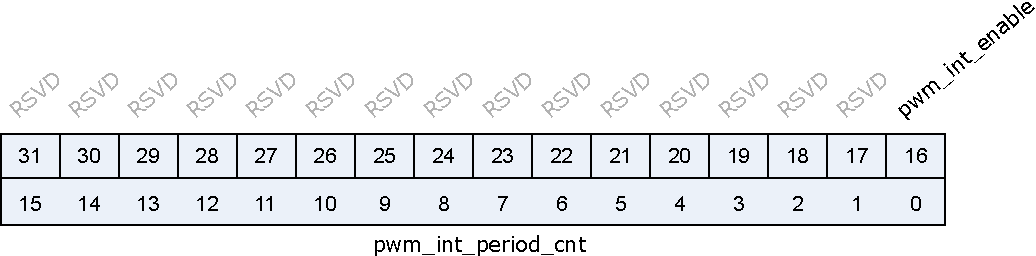
\includegraphics{pwm_pwm4_interrupt.pdf}
\end{figure}

\regdes{31:17&RSVD& & & \\\hline
16&pwm\_int\_enable&r/w&1'b0&PWM interrupt enable\\\hline
15:0&pwm\_int\_period\_cnt&r/w&16'd0&PWM interrupt period counter threshold\\\hline

}
